\documentclass[twocolumn,a4j]{jsarticle}
\setlength{\topmargin}{-20.4cm}
\setlength{\oddsidemargin}{-10.4mm}
\setlength{\evensidemargin}{-10.4mm}
\setlength{\textwidth}{18cm}
\setlength{\textheight}{26cm}

\usepackage[top=15truemm,bottom=20truemm,left=20truemm,right=20truemm]{geometry}
\usepackage[latin1]{inputenc}
\usepackage{amsmath}
\usepackage{amsfonts}
\usepackage{amssymb}
\usepackage[dvipdfmx]{graphicx}
\usepackage[hang,small,bf]{caption}
\usepackage[subrefformat=parens]{subcaption}
\usepackage[dvipdfmx]{color}
\usepackage{listings}
\usepackage{listings,jvlisting}
\usepackage{geometry}
\usepackage{framed}
\usepackage{color}
\usepackage[dvipdfmx]{hyperref}
\usepackage{ascmac}
\usepackage{enumerate}
\usepackage{tabularx}
\usepackage{cancel}
\usepackage{scalefnt}
\usepackage{overcite}
\usepackage{otf}
\usepackage{multicol}
\usepackage[geometry]{ifsym}
\usepackage{array}

\renewcommand{\figurename}{Fig.}
\renewcommand{\tablename}{Table }

\lstset{
basicstyle={\ttfamily},
identifierstyle={\small},
commentstyle={\smallitshape},
keywordstyle={\small\bfseries},
ndkeywordstyle={\small},
stringstyle={\small\ttfamily},
frame={tb},
breaklines=true,
columns=[l]{fullflexible},
xrightmargin=0zw,
xleftmargin=3zw,
numberstyle={\scriptsize},
stepnumber=1,
numbersep=1zw,
lineskip=-0.5ex
}

% キャプション後ろのダブルコロンを消す
\makeatletter
\long\def\@makecaption#1#2{%
  \vskip\abovecaptionskip
  \iftdir\sbox\@tempboxa{#1\hskip1zw#2}%
    \else\sbox\@tempboxa{#1 #2}%
  \fi
  \ifdim \wd\@tempboxa >\hsize
    \iftdir #1\hskip1zw#2\relax\par
      \else #1 #2\relax\par\fi
  \else
    \global \@minipagefalse
    \hbox to\hsize{\hfil\box\@tempboxa\hfil}%
  \fi
  \vskip\belowcaptionskip}
\makeatother

% タイトル
\makeatletter
\def\@maketitle
{
\begin{center}
{\LARGE \@title \par}
\end{center}
\begin{flushright}
{\large \@date 報告書 No.35}\\
{\large M2 \@author}
\end{flushright}
\par\vskip 1.5em
}
\makeatother

\author{来代 勝胤}
\title{令和4年度 10月 第1週 報告書}
\date{2022/10/3}

\begin{document}
\columnseprule=0.1mm
\maketitle

\section*{報告内容}
\begin{enumerate}[1.]
  \item マッチングアルゴリズムの検討
  \item 来週の予定
\end{enumerate}

\section{マッチングアルゴリズムの検討}

\subsection{クラスターデータ}
\begin{figure}[htbp]
  \centering
  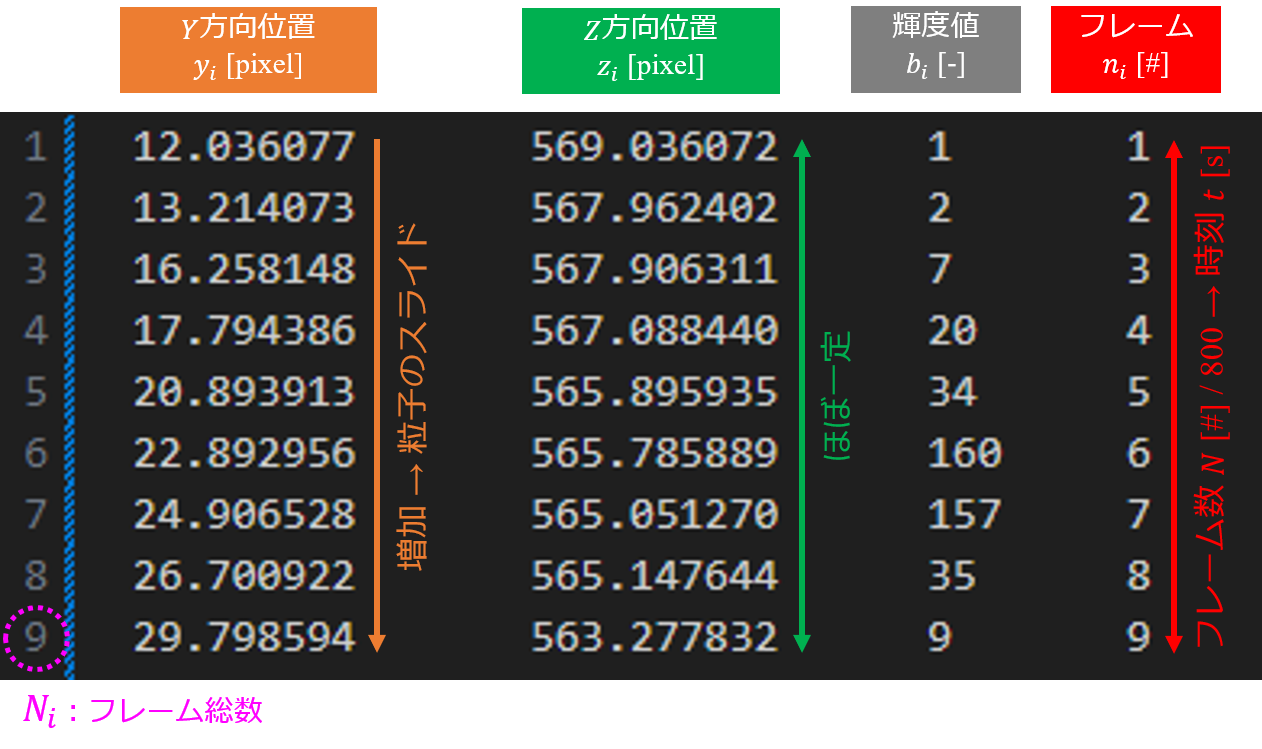
\includegraphics[width=80mm]{../images/cluster_data.png}
  \caption{Cluster data of a blue particle}
\end{figure}

$\blacksquare$\;\gt{粒子位置の計算}
\begin{eqnarray*}
  y'_i = \frac{1}{N_i} \sum_{j=1}^{N} y_{ij} &:& y方向位置  \\
  z'_i = \frac{1}{N_i} \sum_{j=1}^{N} z_{ij} &:& z方向位置  \\
  n'_i = \frac{1}{N_i} \sum_{j=1}^{N} n_{ij} &:& フレーム数 \\
  i &:& \text{クラスタ番号}\\
  j &:& \text{フレーム番号}\\
  N_i &:& i
\end{eqnarray*}

$\blacksquare$\;\gt{主流方向速度の推定}
\begin{eqnarray*}
  u_i &=& T \times \frac{f}{N_i}\\
  T &:& \text{レーザーシート厚み} \\
  f &:& \text{フレームレート}\\
\end{eqnarray*}

\newpage
\subsection{ユークリッド距離によるニアレストマッチング}
$\blacksquare$\;\gt{三角翼右翼後流の計測結果}
\begin{figure}[htbp]
  \centering
  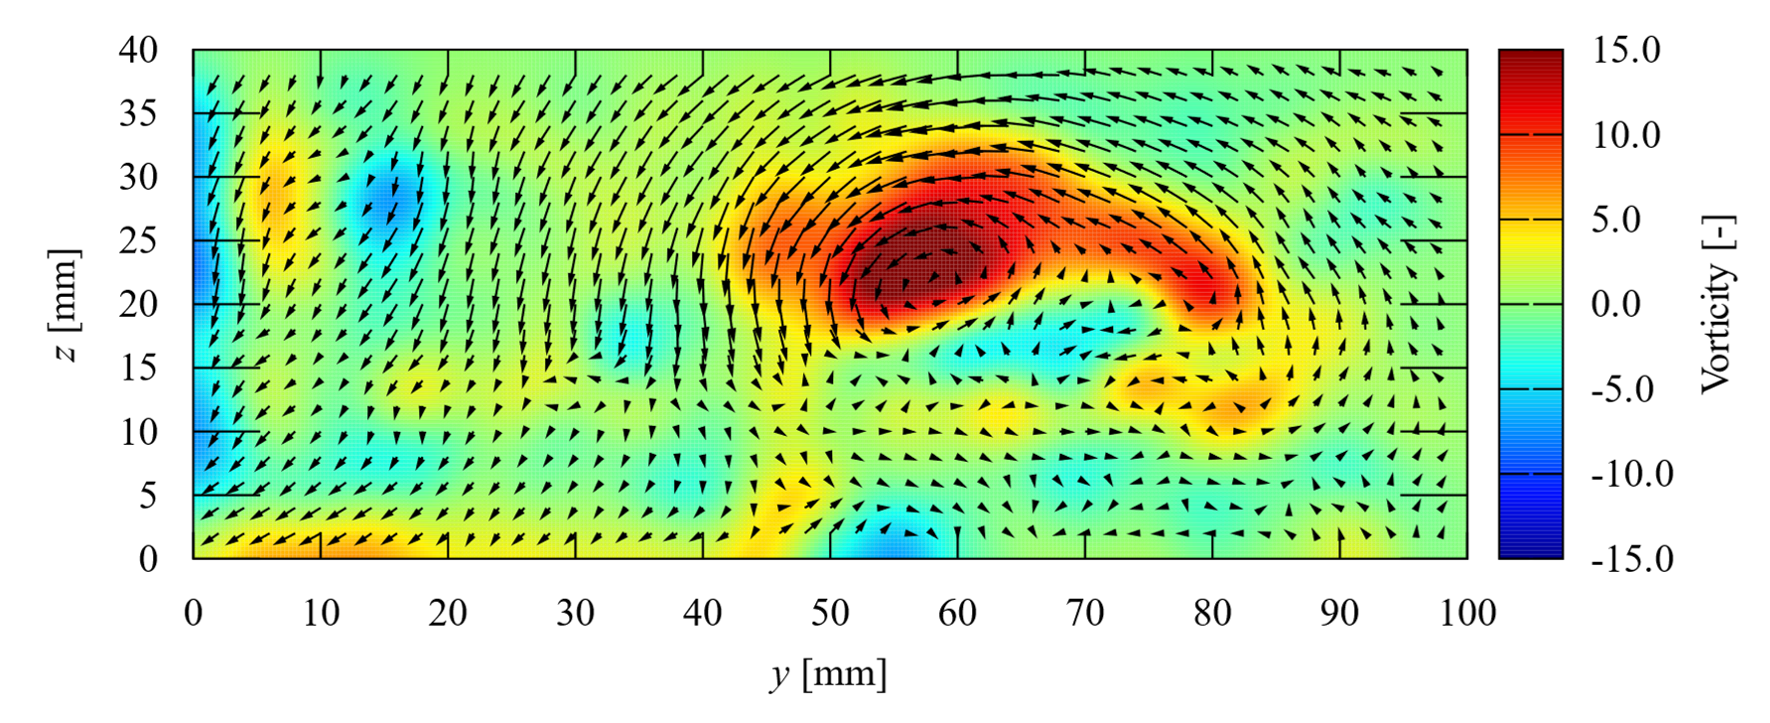
\includegraphics[width=90mm]{../images/vorticity.png}
  \caption{Velocity vector field and vorticity field}
  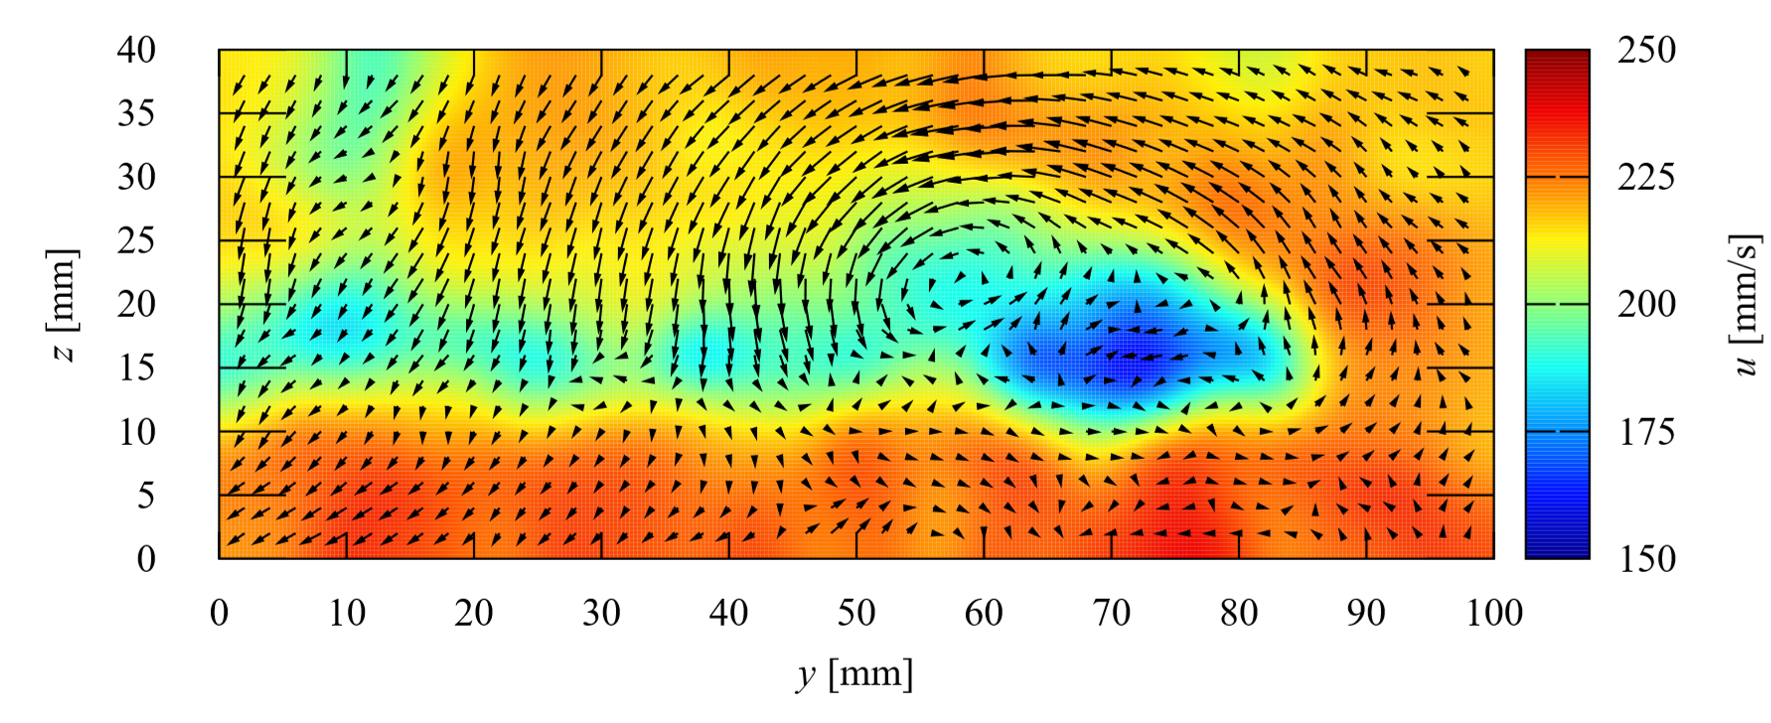
\includegraphics[width=90mm]{../images/velocity.png}
  \caption{Velocity vector field and $u$}
\end{figure}

\subsection{直線どおしの最短距離を用いたマッチング}
$\blacksquare$\;\gt{3次元直線式}
\begin{eqnarray*}
  n = a y + b z + c
\end{eqnarray*}

$\blacksquare$\;\gt{三角翼右翼後流の計測結果:失敗}
\begin{figure}[htbp]
  \centering
  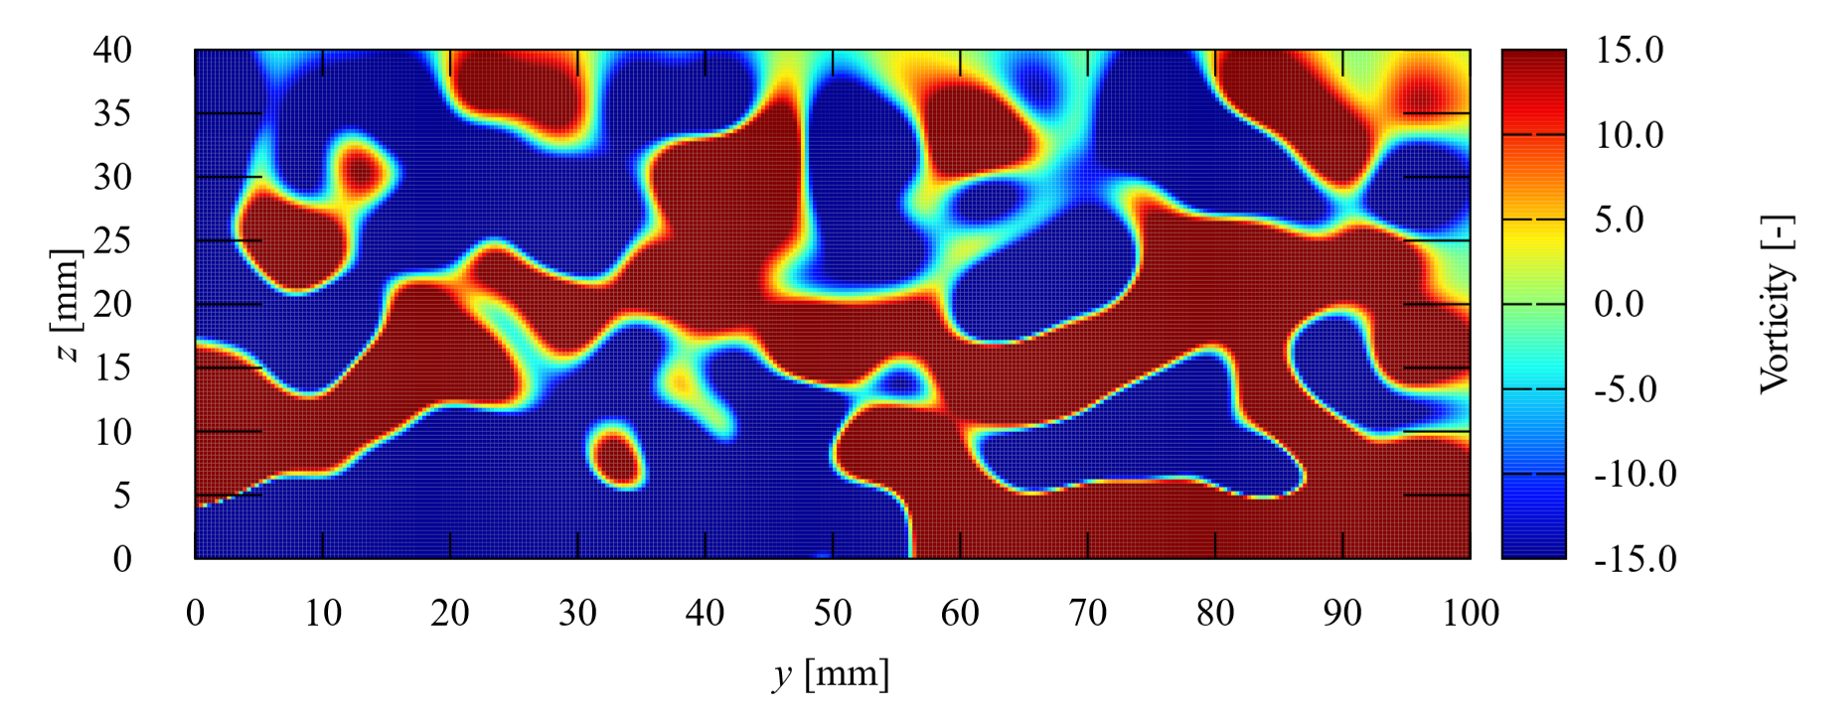
\includegraphics[width=90mm]{../images/vorticity_miss.png}
  \caption{Velocity vector field and vorticity field}
\end{figure}

\section{来週の予定}
\begin{itemize}
  \item マッチングアルゴリズムの検討 (続き)
\end{itemize}

\end{document}